% $Header: /cvsroot/latex-beamer/latex-beamer/solutions/generic-talks/generic-ornate-15min-45min.en.tex,v 1.5 2007/01/28 20:48:23 tantau Exp $

\documentclass[12pt]{beamer}
%\documentclass[12pt,handout]{beamer}

% This file is a solution template for:

% - Giving a talk on some subject.
% - The talk is between 15min and 45min long.
% - Style is ornate.



% Copyright 2004 by Till Tantau <tantau@users.sourceforge.net>.
%
% In principle, this file can be redistributed and/or modified under
% the terms of the GNU Public License, version 2.
%
% However, this file is supposed to be a template to be modified
% for your own needs. For this reason, if you use this file as a
% template and not specifically distribute it as part of a another
% package/program, I grant the extra permission to freely copy and
% modify this file as you see fit and even to delete this copyright
% notice.


\mode<presentation>
{
  \usetheme{default}
  % or ...

  \setbeamercovered{transparent}
  % or whatever (possibly just delete it)
}
\setbeamertemplate{navigation symbols}{}%remove navigation symbols


\usepackage[english]{babel}
% or whatever

\usepackage[latin1]{inputenc}
% or whatever

\usepackage{times}
\usepackage{sansmathfonts}
\usepackage[T1]{fontenc}
% Or whatever. Note that the encoding and the font should match. If T1
% does not look nice, try deleting the line with the fontenc.


\title%[Short Paper Title] % (optional, use only with long paper titles)
{}

\subtitle
{} % (optional)

\author%[Author, Another] (optional, use only with lots of authors)
{Ben Holder}%{F.~Author\inst{1} \and S.~Another\inst{2}}
% - Use the \inst{?} command only if the authors have different
%   affiliation.

%\institute[Universities of Somewhere and Elsewhere] % (optional, but mostly needed)
%{
%  \inst{1}%
%  Department of Computer Science\\
%  University of Somewhere
%  \and
%  \inst{2}%
%  Department of Theoretical Philosophy\\
%  University of Elsewhere}
%% - Use the \inst command only if there are several affiliations.
%% - Keep it simple, no one is interested in your street address.

\date%[Short Occasion] % (optional)
{}

\subject{Talks}
% This is only inserted into the PDF information catalog. Can be left
% out.



% If you have a file called "university-logo-filename.xxx", where xxx
% is a graphic format that can be processed by latex or pdflatex,
% resp., then you can add a logo as follows:

% \pgfdeclareimage[height=0.5cm]{university-logo}{university-logo-filename}
% \logo{\pgfuseimage{university-logo}}



% Delete this, if you do not want the table of contents to pop up at
% the beginning of each subsection:
%\AtBeginSubsection[]
%{
%  \begin{frame}<beamer>{Outline}
%    \tableofcontents[currentsection,currentsubsection]
%  \end{frame}
%}


% If you wish to uncover everything in a step-wise fashion, uncomment
% the following command:

%\beamerdefaultoverlayspecification{<+->}

\usepackage{enumerate}
\usepackage{amsmath}
\usepackage{amssymb}
\usepackage[amssymb]{SIunits}
\usepackage{url}
\usepackage{hyperref}
\usepackage[normalem]{ulem}


\setbeamercovered{invisible}

\hypersetup{
    colorlinks=true,     % false: boxed links; true: colored links
    linkcolor=red,       % color of internal links
    citecolor=blue,      % color of links to bibliography
    filecolor=blue,      % color of file links
    urlcolor=blue        % color of external links
}


\begin{document}

%\begin{frame}
%  \titlepage
%\end{frame}

%%%%%%%%%%%%%%%%%%%%%%%%%%%%%%%%%%%%%%
\begin{frame}{Announcements}
	%
	\begin{itemize}
	\addtolength{\itemsep}{0.5\baselineskip}
	\item Any questions/issues?
	\item \underline{Schedule}:
		%
		\begin{itemize}
		\item[]{\bf Today (Follow-up)}: Discussion Q2 (absorption lines); Discussion Q3 ({\bf now a bonus question})
		\item[]{\bf Today (Follow-up)}: Boiling Lab --- what did we observe and what does it mean?
		\item[]{\bf Today (Follow-up)}: Where are we on $T_\text{Earth}$?
		\item[]{\bf Today (New)}: Why is there evaporation below boiling?
		\item[]{\bf Tomorrow (Lab)}: Evaporation of water and clouds!
		\item[]{\bf Thursday (Discussion)}: Final calculation of Earth's equilibrium temperature.
		\item[] {\bf Next Week}: \underline{No Lab}; Starting paleo perturbations of temperature.
		\end{itemize}
		%
	\end{itemize}

\end{frame}
%%%%%%%%%%%%%%%%%%%%%%%%%%%%%%%%%%%%%%
\begin{frame}{Today's Reading Quiz (3 min)}


	
\vspace{1cm}

On your own sheet of paper\ldots

\vspace{0.5cm}

{\bf Say a few words about each: {\em atmospheric pressure}, {\em humidity of air}, {\em latent heat}.}

\vspace{0.5cm}

Turn in to Blackboard as scanned pdf (or image is fine).

\end{frame}
%%%%%%%%%%%%%%%%%%%%%%%%%%%%%%%%%%%%%%
\begin{frame}{Question 2 from Discussion}

\begin{center}
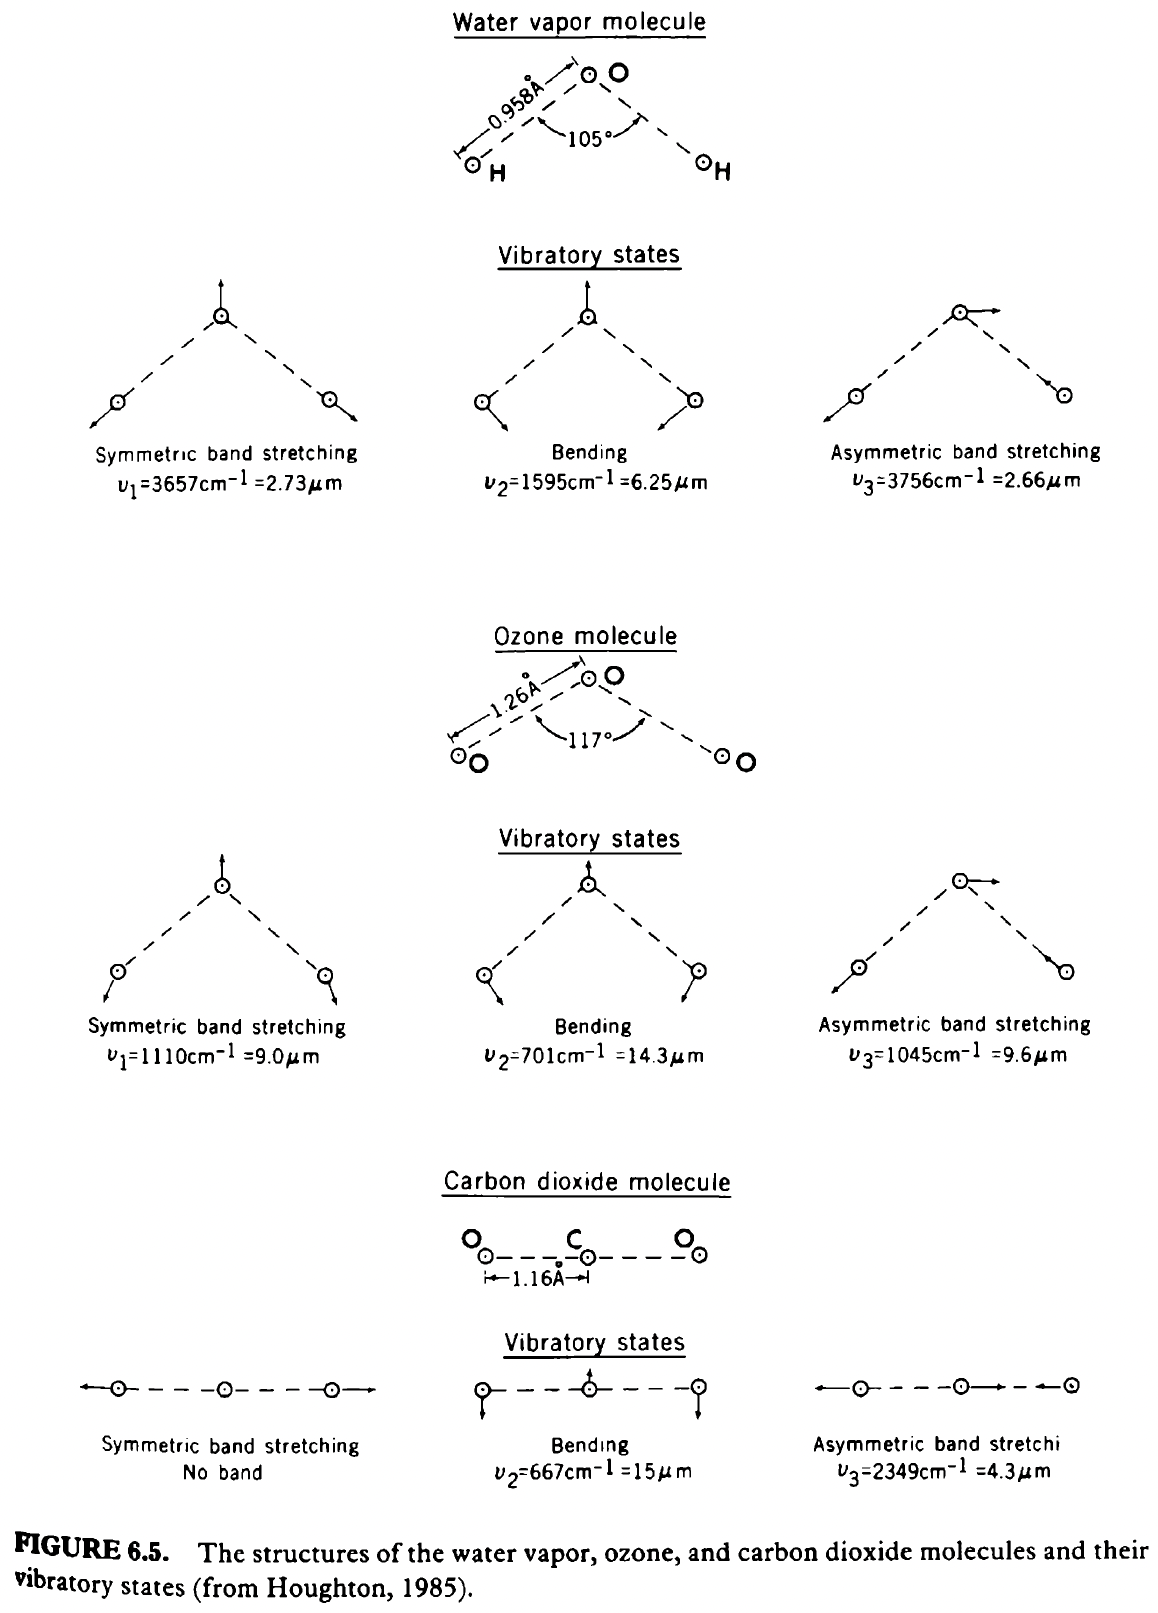
\includegraphics[width=0.55\textwidth]{images/peixoto_fig6-5_structure-water-ozone-co2.png}
\end{center}

\end{frame}
%%%%%%%%%%%%%%%%%%%%%%%%%%%%%%%%%%%%%%
\begin{frame}{Question 3 from Discussion}

\begin{center}
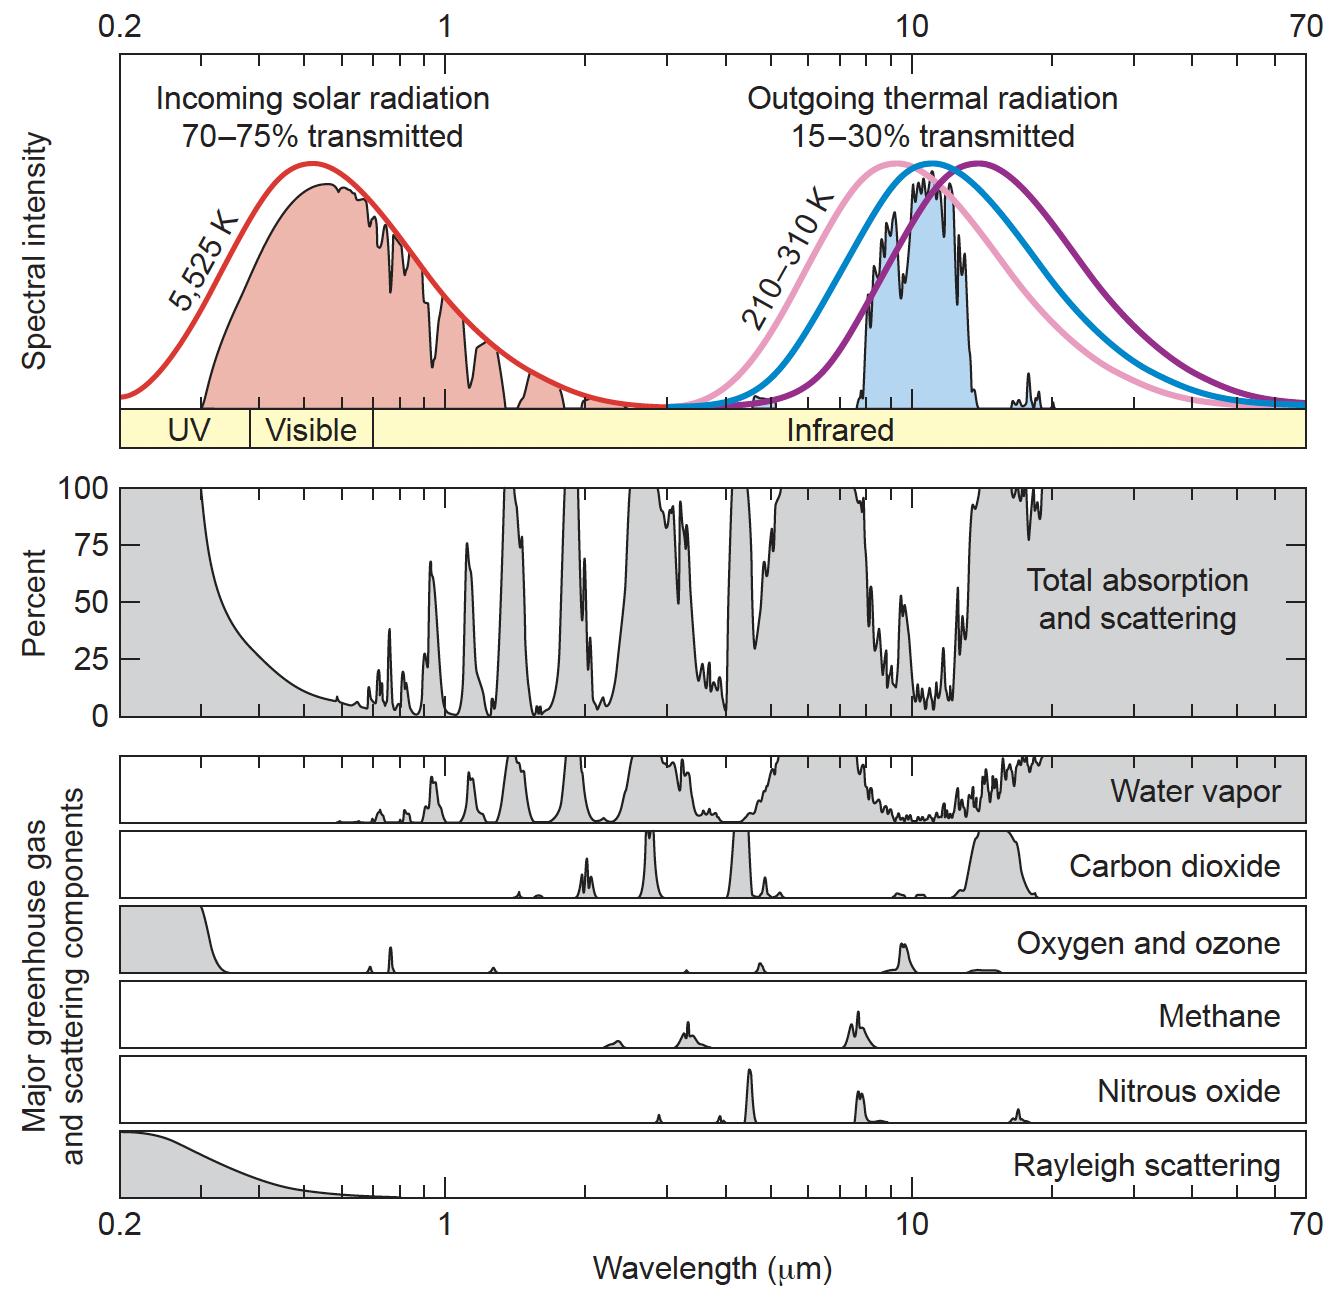
\includegraphics[width=0.8\textwidth]{images/atmospheric-absorption-transmission_rohde_mathez-textbook_no-caption.png}
\end{center}



\end{frame}
%%%%%%%%%%%%%%%%%%%%%%%%%%%%%%%%%%%%%%
\begin{frame}{Boiling Lab: Data}


\begin{center}
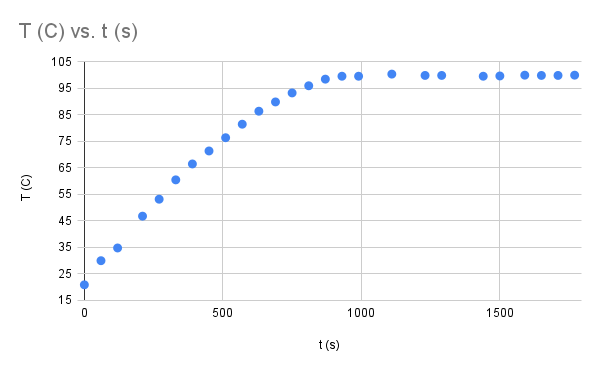
\includegraphics[width=0.55\textwidth]{images/temp-vs-time_boiling-trial-1.png}\\
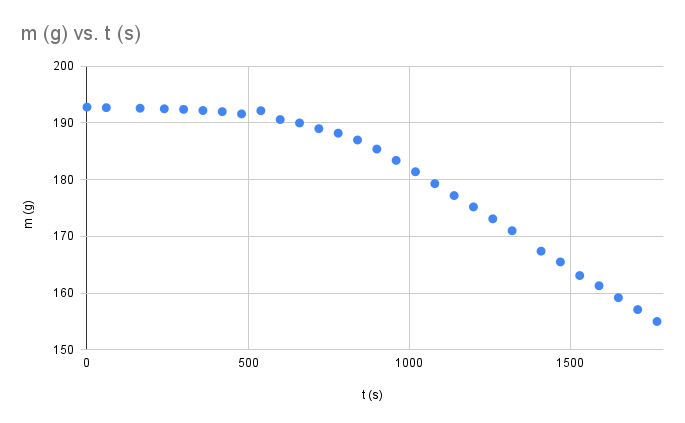
\includegraphics[width=0.55\textwidth]{images/mass-vs-time_boiling-trial-1.png}\\
\end{center}


\end{frame}
%%%%%%%%%%%%%%%%%%%%%%%%%%%%%%%%%%%%%%
\begin{frame}{Boiling Lab: Analysis}

Let's calculate the {\em latent heat of vaporization}, $L_v$, knowing that the specific heat capacity of water is \unit{4.2}{\joule/\gram\kelvin}.

\begin{center}
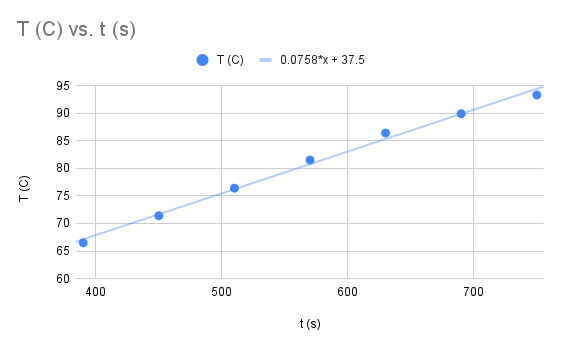
\includegraphics[width=0.55\textwidth]{images/temp-vs-time_boiling-trial-1_fit.png}\\
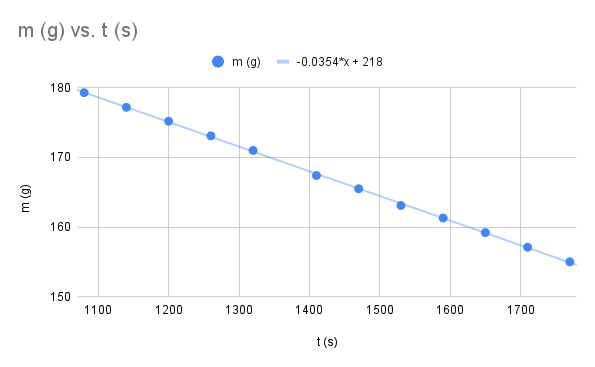
\includegraphics[width=0.55\textwidth]{images/mass-vs-time_boiling-trial-1_fit-after-boiling.png}
\end{center}


\end{frame}
%%%%%%%%%%%%%%%%%%%%%%%%%%%%%%%%%%%%%%
\begin{frame}{Boiling Lab: Analysis (2nd Attempt)}


\begin{center}
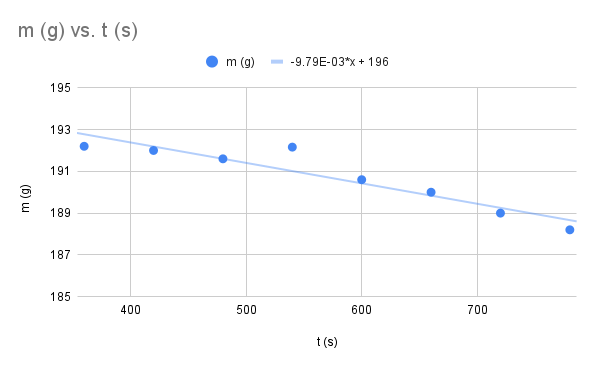
\includegraphics[width=0.7\textwidth]{images/mass-vs-time_boiling-trial-1_fit-before-boiling.png}
\end{center}

\vspace{6cm}


\end{frame}
%%%%%%%%%%%%%%%%%%%%%%%%%%%%%%%%%%%%%%
\begin{frame}{Phase Transitions in (Pure) Water}

\begin{center}
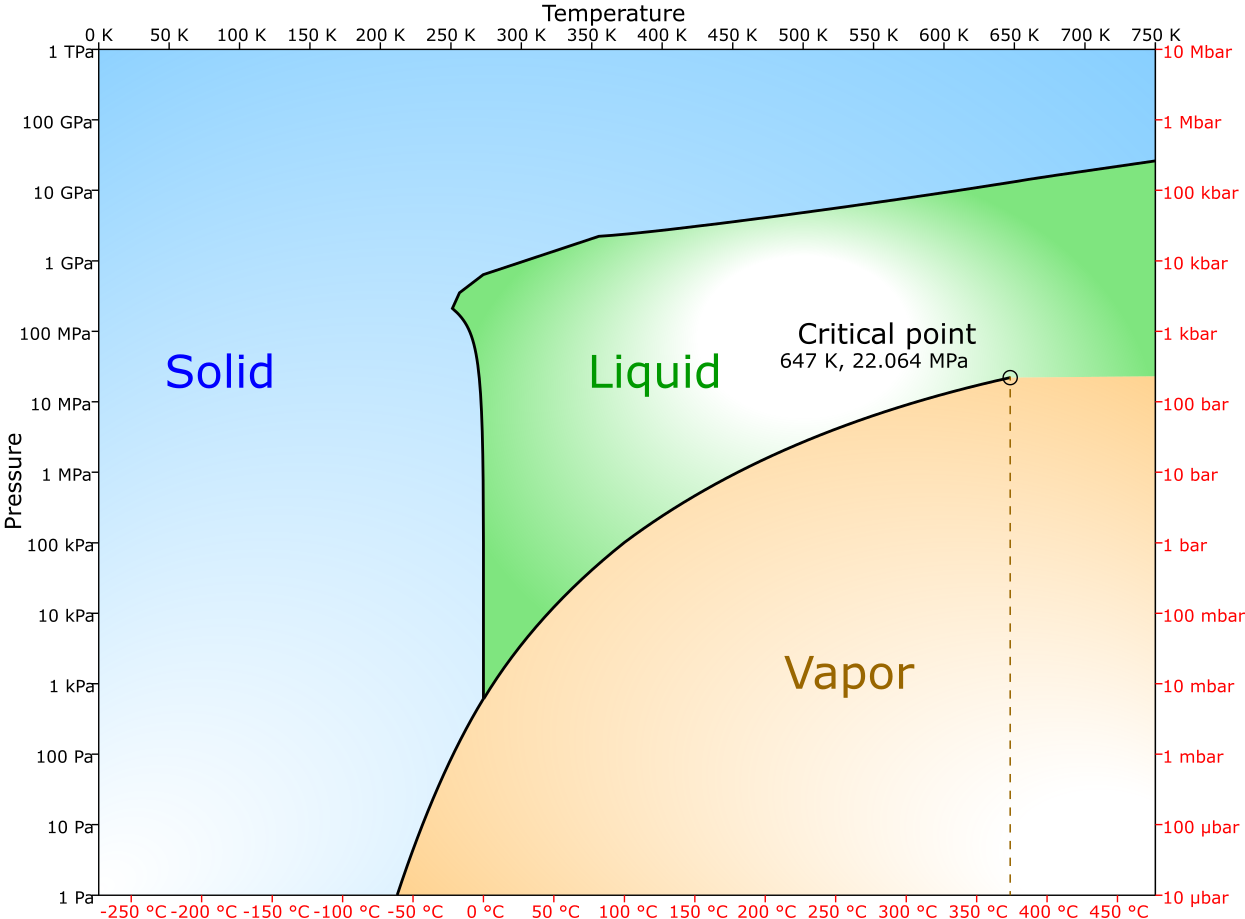
\includegraphics[width=\textwidth]{images/07_phase-diagram-of-water-simplified_wikimedia-Cmglee_edited.png}
\end{center}



\end{frame}
%%%%%%%%%%%%%%%%%%%%%%%%%%%%%%%%%%%%%%
\begin{frame}{Water Evaporation in Air}

Consider this figure from the {\em Mathez} textbook reading today:

\begin{center}
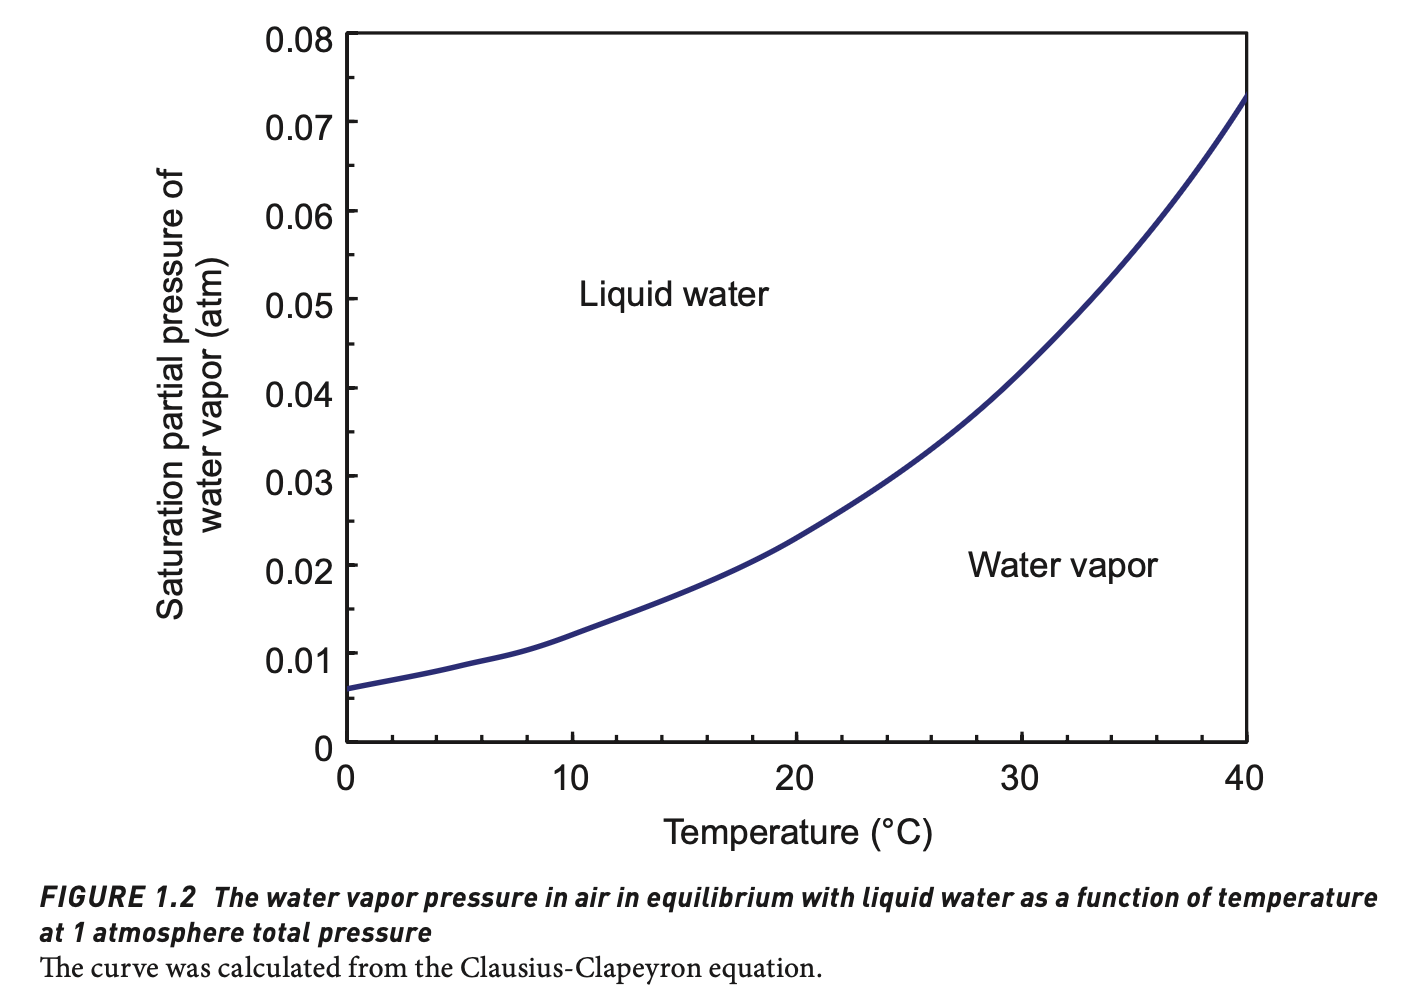
\includegraphics[width=0.8\textwidth]{images/liquid-vapor-transition-air_mathez_fig1-2.png}
\end{center}

Why are the values of the pressure so different along the line of transition from liquid to vapor?


\end{frame}
%%%%%%%%%%%%%%%%%%%%%%%%%%%%%%%%%%%%%%
\begin{frame}{Water Evaporation in Air}

Answer: Because evaporation in air uses the so-called {\bf partial pressure} of water within the whole air:
	%
	\begin{equation*}
	p_\text{partial, $\text{H}_2\text{O}$}  = \frac{\text{moles}_\text{\,$\text{H}_2\text{O}$}}{\text{moles}_{\, \text{air}}} \times p_\text{atm}
	\end{equation*}
	%
Where $p_\text{atm} = \unit{101}{\kilo\pascal} = \unit{1}{atm}$ is the full atmospheric pressure. Typically the mole fraction above is a few percent.  Let's try with 2\% \ldots what is the new boiling point?

\vspace{4cm}


\end{frame}
%%%%%%%%%%%%%%%%%%%%%%%%%%%%%%%%%%%%%%
\begin{frame}{Calculating the equilibrium  $T_\text{Earth}$}

Recall our steps to calculate the equilibrium temperature of Earth thus far:
	%
	\begin{itemize}
	\item Planet with no atmosphere, receiving solar radiation from the sun at $S / 4 (1 - \alpha)$
	\item Planet receiving that solar radiation, with an atmosphere.
	\end{itemize}
	%
Now (in Discussion this week) we will make one final adjustment:
	%
	\begin{itemize}
	\item Planet with an atmosphere, plus transport of water vapor above the greenhouse gas layer.
	\end{itemize}
	
	\vspace{4cm}




\end{frame}
%%%%%%%%%%%%%%%%%%%%%%%%%%%%%%%%%%%%%%
\end{document}
